\documentclass[11pt]{article}
\setlength{\topmargin}{-.5in}
\setlength{\textheight}{23.5cm}
\setlength{\textwidth}{17.0cm}
\setlength{\oddsidemargin}{.025in}
\setlength{\evensidemargin}{.025in}
\setlength{\textwidth}{6.25in}
\usepackage{amsmath}
\usepackage{graphicx}
\usepackage{verbatim}   % useful for program listings
\usepackage{color}      % use if color is used in text
\usepackage{subfigure}  % use for side-by-side figures
\begin{document}
\begin{titlepage}
\begin{center}
\textsc{ \LARGE Expanding QTL analysis \\}
\textsc{High performance computing of QTLs for experimental crosses\\}
\end{center}
$ $\\
\\\\\\\\\\\\\\\\
\\\\\\\\\\\\\\\\
\\\\\\\\\\\\\\\\
\\\\\\\\\\\\\\\\
\\\\\\\\\\\\\\\\
\begin{minipage}{0.5\textwidth}
  \begin{flushleft} \large
  \emph{Author:}\\
  Danny \textsc{Arends}\\
  $ $\\
  $ $\\
  \end{flushleft}
  \end{minipage}
  \begin{minipage}{0.5\textwidth}
  \begin{flushright} \large
  \emph{Supervision:} \\
  Dr. Pjotr \textsc{Prins}\\
  Dr. Ritsert \textsc{Jansen}\\
  Dr. Karl \textsc{Broman}\\
  \end{flushright}
\end{minipage}

\end{titlepage}
\input{Abstract.tex}
\newpage
\section*{Terms \& Abbreviations}
\begin{itemize}
	\item API - Application programming interface 
	\item AIC - Akaike's information criterion
	\item BC - Backcross (Specialized animal breeding technique)
  \item (M)Bp - (Mega)Basepair
	\item CIM - Composite interval mapping
	\item cM - centiMorgan
  \item CPU - Central processing unit
  \item Core - A single processing unit on a CPU
	\item F2 - F2 intercross (Specialized animal breeding technique)
  \item GPU - Graphics processing unit
  \item GWAS - Genomewide association study
	\item HPC(/V) - High performance computing (and visualisation)
	\item LCMS - Liquid chromatography-mass spectrometry
	\item LOD - -10Log(Pvalue) so a lod score of 3 means a chance of a 1000 : 1
  \item Molgenis - Molecular genetics information system
	\item MQM - Multiple QTL mapping \cite{jansen93}
	\item PBS - Portable Batch System \cite{PBS2000}
	\item QTL - Quantative Trait Locus
	\item eQTL - QTL associated with gene expression
	\item pQTL - QTL associated with protein abundance
	\item mQTL - QTL associated with metabolites
  \item R - Statistical programming language and environment
  \item R/qtl - R-package by Prof. K. Brohman
  \item RIL - Recombinant inbred line (Specialized animal breeding technique)
	\item RUG - University of Groningen
  \item SNOW - Simple Network of Workstations \cite{tierney04}
	\item XGAP - eXtensable Genotype And Phenotype dataplatform
\end{itemize}

\section{Introduction}
\subsection{r/qtl}
R/qtl is an open source package for mapping QTL in experimental crosses for the R programming language\cite{broman09}\cite{broman03}.
It can be used to analyse several types of experimental crosses (Backcross (BC), F2, Recombinant inbred lines (RIL), Intercrosses (IC)) 
. Furthermore it offers many methods for QTL mapping (Composite interval mapping (CIM), expectation maximization (EM), marker regression (MR) and 
Extended Haley-Knot (eHK)). Because R/qtl supports different experimental crosses and contains many extra functions (plotting, genotype checking, etc).
Because it is opensource software no cost are associated with usage of the R-package (or the R-software infrastructure). Also its opensource nature
 makes it easy for others to contribute to the package. 
Our goal is to make complex QTL mapping methods widely accessible and allow users to focus on modeling rather than computing. R/qtl 
is becoming an increasingly popular environment for QTL analysis and has its own stabile userbase\cite{broman03}.
\subsection{Molgenis \& XGAP}
Storing information is very important, it becomes even more crucial when large -omics datasets are involved. These -omics sets are ussually generated 
in plain text format and read into a database system (mySQL/Oracle/msSQL). However these systems are not tailored to the needs of this biological data.
Providing ussually only storage for the most basic of datatypes (integers,strings,etc), they ussually lack biological dataformats, but are very good 
at storing data within a strict format. The molgenis database system using the extensible genotype \& phenotype (XGAP) datamodel aims to solve both these problem.
It does so by providing an easy to change datamodel (XGAP), with a generator to change the currentdatabase layout with a push of the button. The adaptability
of the system allows for easy managment of constantly changing biological data. This is furthermore enhanched by allowing for 3th party plugin to be 
connected to the database system. Molgenis was used in our project as out dataproviding software and a plugin was designed and implemented to enable 
molgenis users to perform R/QTL analysis from a webenviroment.
\subsection{High Performance Computing (HPC)}
The university of Groningen has an institute dedicated to high performance computing. The cluster is comprised of 168 machines running on a dualcore CPU. To 
facilitate high performance computations a PBS\cite{PBS2000} jobsceduler is present on the cluster, together with an installation of R-2.9.0. When computational job become too big for a desktop computer, these HPC facilities can be used. 
Another part of the project was focused on using the high speed computing facilities available in combination with the molgenis database system. 
\section{Materials and Infrastructure}
\subsection{Cluster infrastructure}
To analyse QTL's directly from a molgenis webenviroment, additional calculation power is needed to perform these intensive calculations. 
Because QTL calculation can take upto (or more) than 24 hours these calculations should be performed by a seperate machine 
or even a parallel processing cluster. The plugin created uses and SHH tunnel to a machine running a PBS job sceduler, any machine using PBS to scedule jobs  
can in theory be used when the following prerequisites are met:
\begin{itemize}
	\item Connection via SHH using login and password
	\item installed PBS job sceduling system (qsub, qstat, qselect, qdel) \cite{qstat06}
	\item R 2.8.0+
	\item R Packages: RCurl, molgenis, R/qtl (optional: SNOW)
\end{itemize}
\section{Method}
\subsection{Datastructuring and storage}
In R we adopted the R/qtl cross object format, however when sharing results with others 
(publication, etc) this binary format is not usefull. Here databases can help, storing huge amounts of data like publicly available 
and / or private datasets. Adding data to a database in a transaction based way ensures data consistency. 
Also database systems allow for third party software to store and retrieve data from the database directly or via
a supplied application programming interface (API). The XGAP \cite{morris07} (Xtensible Genotype and Phenotype) datamodel is used 
to format data in a homogenious matter when storing data into a molgenisDB. This XGAP format ensures data 
is extensible and consistent. The molgenisDB system ensures dataconsistency and -coherency, plus allowing easy 
access from R / JAVA / SOAP or by using HTML scripting.
\subsection{HPC of QTLs using molgenis}
A plugin was created to enable users to use the r/qtl package from the molgenis webenviroment. To use this plugin another machine is required 
to distribute jobs and do qtl analysis. This was done to separate qtl calculation from normal server operations.
On this website public datasets are available and the user can use the HPC cluster of the Rijks Universiteit of Groningen to do highperformance qtl analysis.
Also we created an overview of the current infrastructure needed for a functional plugin.
\section{Results}

\subsection{Datastructuring and storage}
Methods to connect R/qtl to XGAP/molgenisDB were writen in the R programming language using the molgenis R-API. 
To use the molgenis API for R an R-package named Rcurl \cite{Rcurl08} is used to make HTTP connections to the 
molgenis server.

\begin{figure}[ht]  
\centering
  \hfill
  \fbox{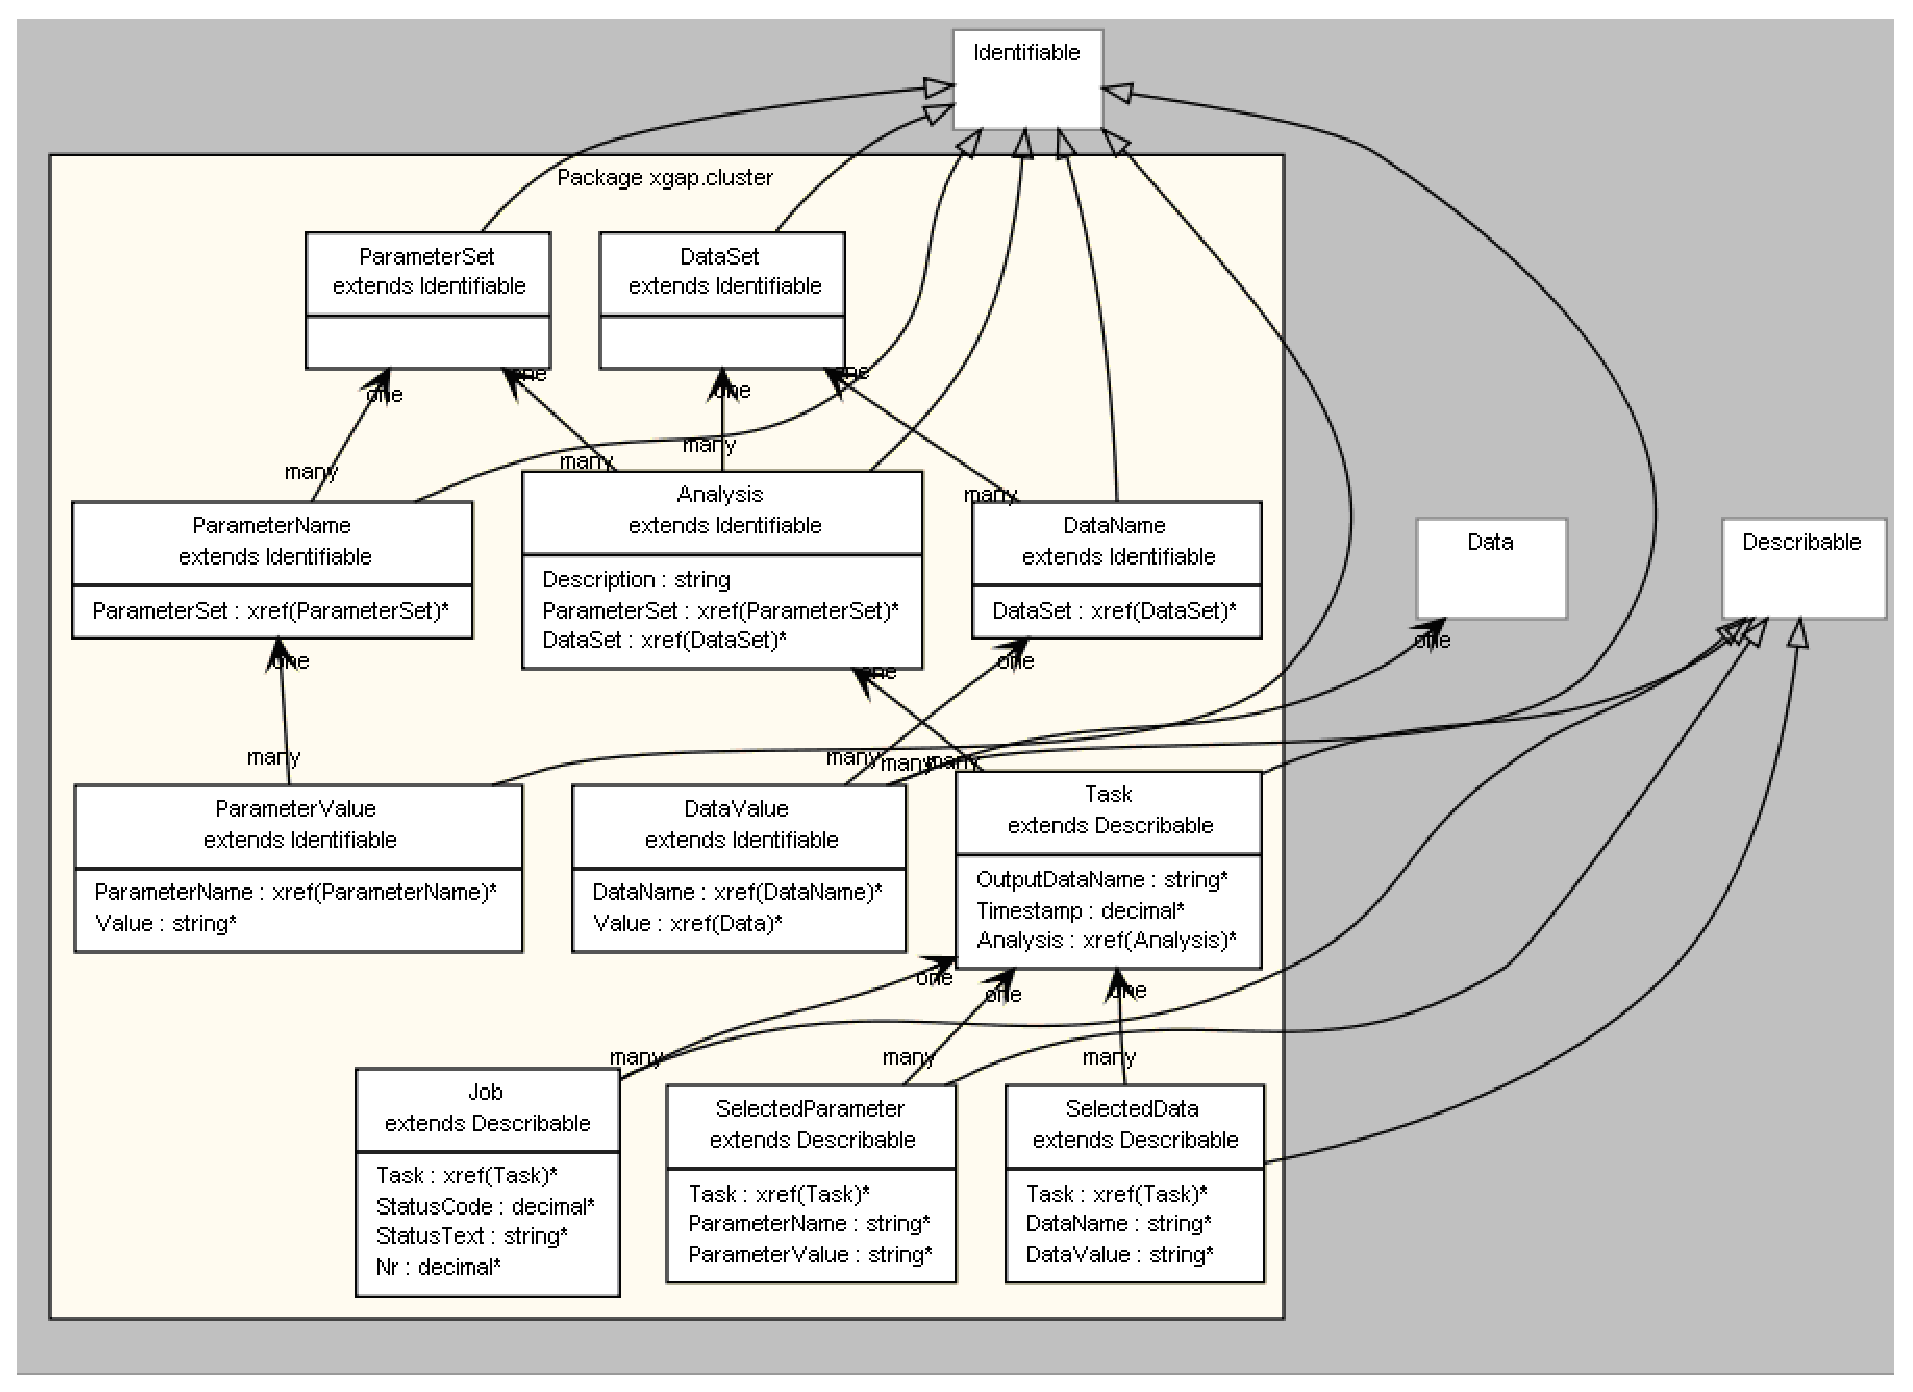
\includegraphics[height=8.0cm,width=15.0cm]{images/datamodel.eps}}
  \caption{Datamodel}
  \label{fig:FigDATAMODEL}    
\end{figure}

\begin{figure}[ht]  
\centering
  \hfill
  \fbox{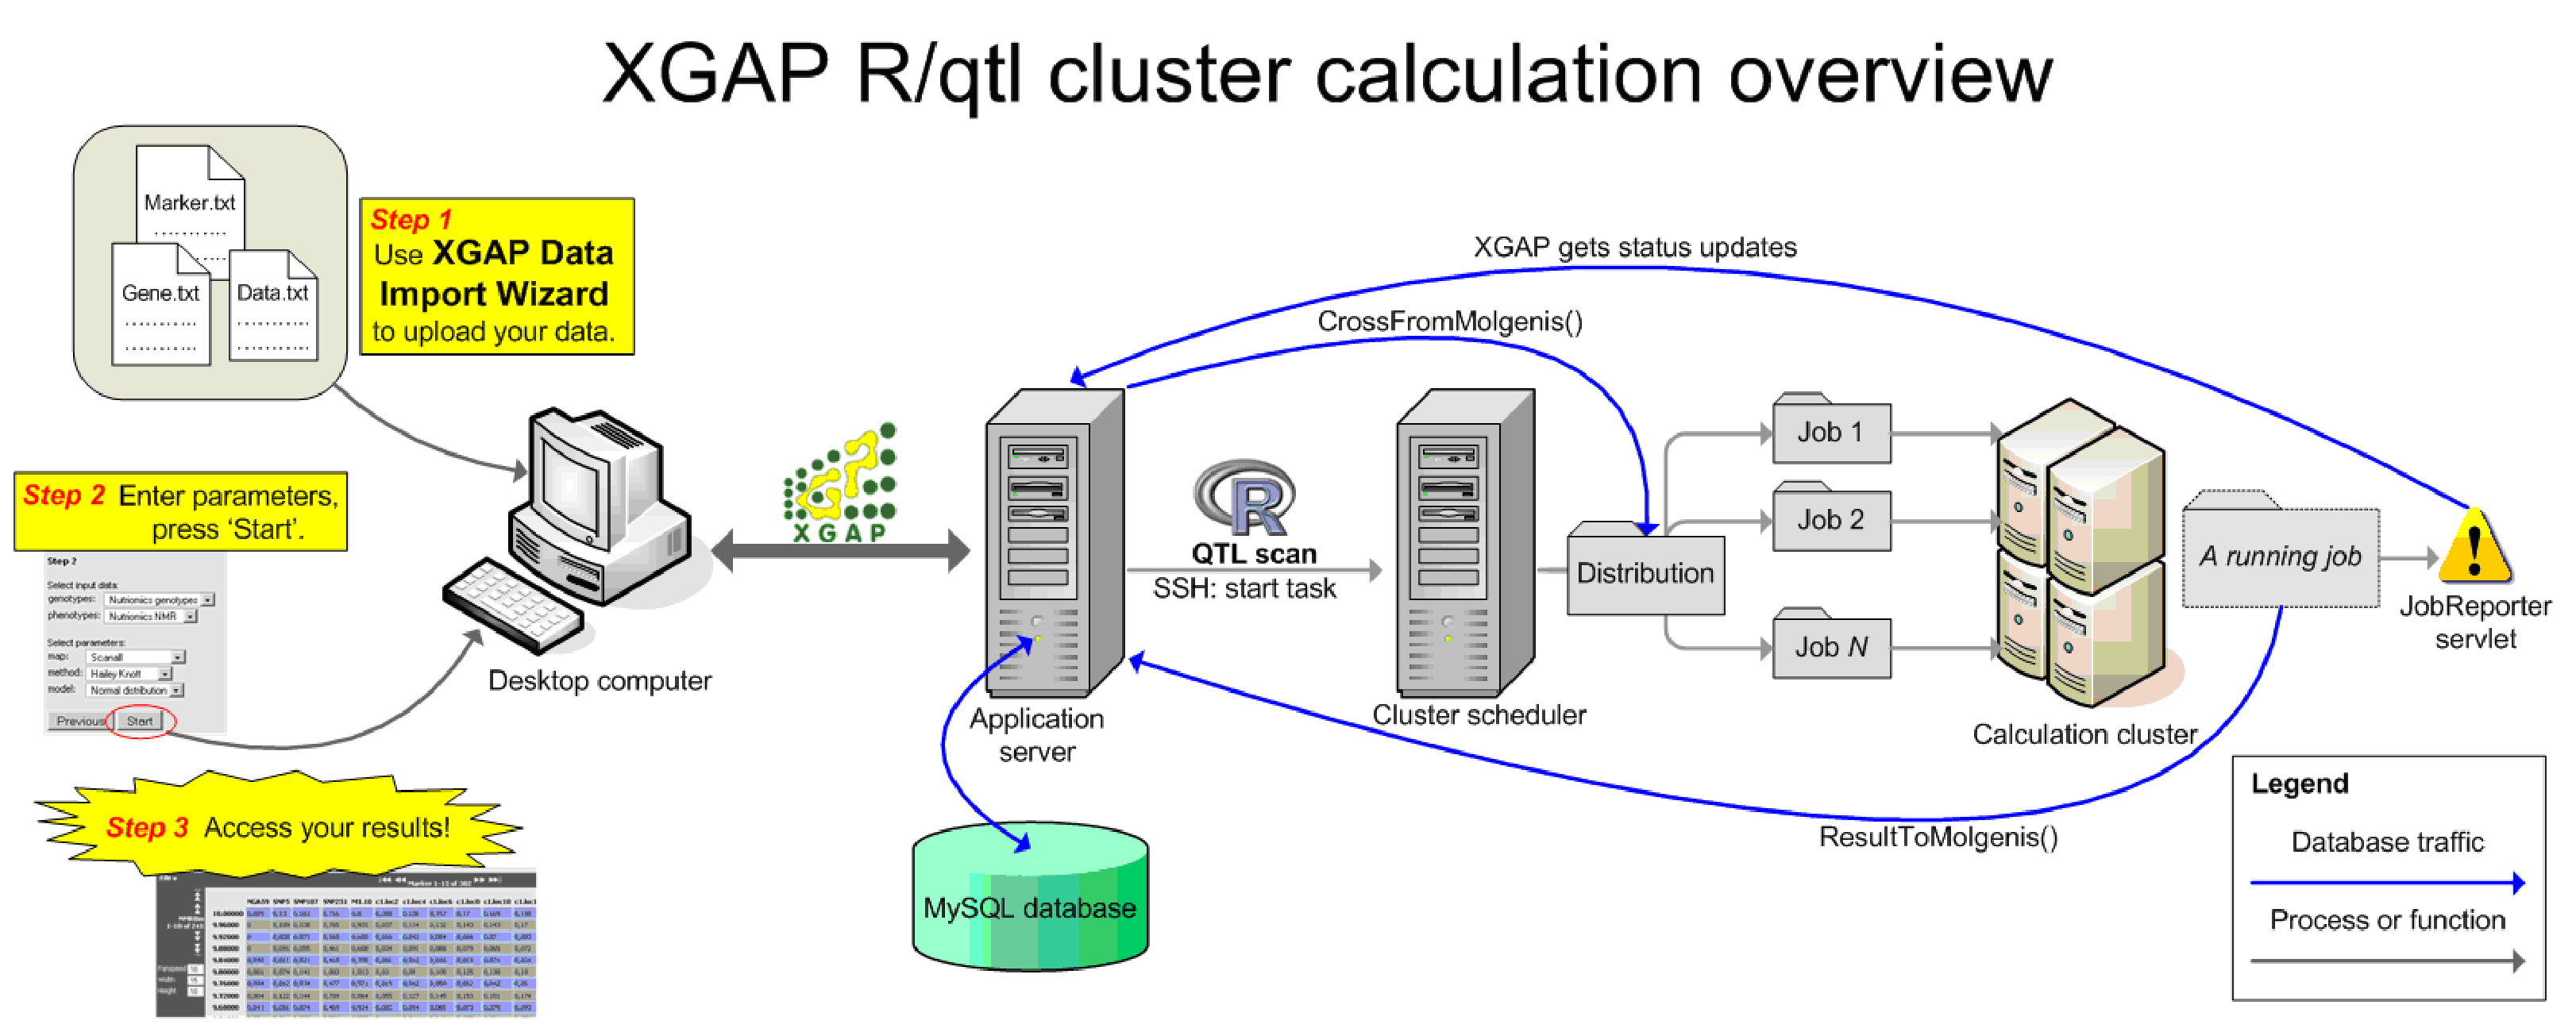
\includegraphics[height=8.0cm,width=15.0cm]{images/layout.eps}}
  \caption{Layout}
  \label{fig:FigLAYOUT}    
\end{figure}

\subsection{HPC of QTLs using molgenis}
Because there is a high threshold for biological users to use R for QTL analysis a webplugin into the molgenis system was created to enable users to 
use the molgenis webinterface to do highspeed parallelized QTL analysis. The plugin stores QTL profiles back into the database and also information about each run.
A webinterface provides users with a one click sollution, while the more complicated task are hidden out of sight. 
An overview of what happens out of sight can be seen in FIG XX.
The following functions are used during cluster analysis
\begin{itemize}
	\item CrossFromMolgenis() - Retrieving a dataset in the R/qtl cross format from a molgenis database system with the XGAP dataformat
	\item ResultsToMolgenis() - Storing results to a molgenis database system with the XGAP dataformat
	\item ResultsFromMolgenis() - Retrieving previously stored QTL analysis results from a molgenis database system with the XGAP dataformat
\end{itemize}

\begin{table}[ht]
	\caption{R/QTL parameters}
	\centering
	\begin{tabular}{| l | c | }
	\hline
	Scanall	&Main scanning interface of R/QTL created by K. Brohman et al\\
			&implementing per marker QTL analysis using different models and mapping methods.\\
	\hline
	MQMall	&Multiple QTL Mapping algorithm created by R.C. Janssen\\
			&implementing multiple QTL modeling and mapping using normal distributions.\\
	\hline
	CIMall	&Composite interval mapping created by G. Churchill and Senuk Sen\\
	\hline
	\end{tabular}
	\label{tbl:tabel0}
\end{table}

\begin{table}[ht]
	\caption{Reporter statuscodes}
	\centering
	\begin{tabular}{| l | c | c | }
	\hline
	-1	&Red	&An error has occurred.\\
	\hline
	0	&Orange	&Submitted to cluster as a potential job.\\
	\hline
	1	&Yellow	&Job is accepted and queued.\\
	\hline
	2	&Blue	&Job calculation done and is now uploading results back to the database.\\
	\hline
	3	&Green	&Job is completed.\\
	\hline
	\end{tabular}
	\label{tbl:tabel1}
\end{table}


\section{Conclusions}
\subsection{HPC of QTLs using molgenis}

\section{Discussion}
\subsection{Datastructuring and storage via: XGAPDB}

\subsection{HPC of QTLs using molgenis}
Further extensions of the plugin currently under development:
\begin{itemize}
	\item - A priori checking of tables selected
	\item - Expose more scanning routines (CIM,MQM)
	\item - Expose all available parameters (scanone,CIM,MQM)
	\item - Better required time estimation of runtime on cluster
	\item - Concurrent runs
	\item - Better status overview using active polling of the calculationserver
\end{itemize}
\newpage
\section{Literature}
 \begin{thebibliography}{9}
 	\bibitem{morris07}
		Swertz MA, Jansen R. C.; 2007
		\emph{Beyond standardization: dynamic software infrastructures for systems biology}
		Nat Rev Genet. 3, 235�243. 
	\bibitem{morris04}
		Swertz M.A., De Brock E.O., Van Hijum S.A., De Jong A., Buist G., Baerends R.J., Kok J., Kuipers O.P., Jansen R.C.; 2004.
		\emph{Molecular Genetics Information System (MOLGENIS): Alternatives in developing local experimental genomics databases}
		Bioinformatics,13, 2075�2083.
	\bibitem{PBS2000}
		Veridian Information Solutions; 2000
		\emph{Portable Batch System - OpenPBS Release 2.3:Administrator Guide}
		website at: www.veridian.com.
	\bibitem{Rcurl08}
		Temple Lang D. ; 2008
		\emph{R as a Web Client � the RCurl package}
		Journal of Statistical Software		
	\bibitem{broman09}
		Broman, K.W.; 2009.
		\emph{A brief tour of R/qtl}
		http://www.rqtl.org, R/qtl tutorials.
	\bibitem{broman03}
		Broman, K.W.; Wu, H.; Sen, S.; Churchill, G.A.; 2003.
		\emph{R/qtl: QTL mapping in experimental crosses}
		Bioinformatics, 19:889-890.
	\bibitem{qstat06}
		The IEEE and The Open Group; 2004.
		\emph{The Open Group Base Specifications Issue 6}
		IEEE Std 1003.1, 2004 Edition
\end{thebibliography}
\newpage
\section{Additional information}
\subsection*{Script \& Code}
Script and code created and used can be found at:\\
http:$\backslash$$\backslash$github.com$\backslash$DannyArends\\
http:$\backslash$$\backslash$github.com$\backslash$DannyArends$\backslash$rqtl-mqm\\
http:$\backslash$$\backslash$github.com$\backslash$DannyArends$\backslash$MolgenisInterface\\

\subsection*{Additional tables}
Tables \ref{tbl:tabel1} \& \ref{tbl:tabelCluster} list the dependencies needed to use the software discribed in this thesis. 
The scriptfile QTLanalysis.R ,dependency for functioning of the clusterservice,
can be found inside the molgenispackage.
Tables \ref{tbl:tabel3} \& \ref{tbl:tabel2} made using R/qtl "Map10" dataset, for scanone bootstrapping parameters were: 
500 bootstraps in batches of 50 at a time on a simulated F2 population with \# individuals as stated in column 1 (Table \ref{tbl:tabel2}).
For mqm we used 50 bootstraps in batches of 5 (Table \ref{tbl:tabel3}). Runs were performed using standard setting for each algorithm. 
Profiling code is available at request.\\

\begin{table}[ht]
	\caption{Requirements for using the R/qtl package}
	\centering
	\begin{tabular}{| l | c | }
	\hline
	Operating system(s):&platform independent\\
	Programming languages:&R, C++\\
	Programs:&R 2.8.0\\
	Dependencies:&SNOW\cite{tierney04}\\
	Published using:&GNU 2 licence\\
	\hline
	\end{tabular}
	\label{tbl:tabel1}
\end{table}

\begin{table}[ht]
	\caption{Requirements for using R/qtl on a cluster}
	\centering
	\begin{tabular}{| l | c | }
	\hline
	Operating system(Cluster):&Unix / Linux\\
	Operating system(Webservice):&platform independent\\
	Programs(Cluster):&R 2.8.0\\
	&PBS\\
	Programs(Webservice):&Molgenis 3.3 Distro\\
	&XGAP 1.1\\
	Dependencies(Cluster):&molgenispackage\\
	&R/qtl\\
	&RCurl\cite{Rcurl08}\\
	&QTLanalysis.R\\
	Dependencies(Webservice):&webserver(APACHE)\\
	&database(mySQL)\\
	&Eclipse Ganymede (Developers)\\
	Published using:&GNU 2 licence\\
	\hline
	\end{tabular}
	\label{tbl:tabelCluster}
\end{table}

\begin{table}[ht]
	\caption{Profiling bootstrap analysis of scanone using a QuadCore machine}
	\centering
	\begin{tabular}{| l | l | l | l | l | c | c | c |}
	\hline
	\# Individuals & Single & Ncore=2 & Ncore=3 & Ncore=4 & \%2vs1 & \%3vs1 & \%4vs1\\
	\hline
	\hline
	10 & 83.00 & 68.00 & 65.00 & 65.00 & -18.1\% & -21.7\% & -21.7\%\\
	20 & 91.00 & 72.00 & 67.00 & 67.00 & -20.9\% & -26.4\% & -26.4\%\\
	50 & 118.00 & 84.00 & 76.00 & 74.00 & -28.8\% & -35.6\% & -37.3\%\\
	100	& 161.00 & 104.00 & 90.00 & 85.00 & -35.4\% & -44.1\% & -47.2\%\\
	200	& 251.00 & 146.00 & 118.00 & 107.00 & -41.8\% & -53.0\% & -57.4\%\\
	350	& 377.00 & 204.00 & 158.00 & 138.00 & -45.9\% & -58.1\% & -63.4\%\\
	500	& 501.00 & 261.00 & 198.00 & 169.00 & -47.9\% & -60.5\% & -66.3\%\\
	750	& 709.00 & 359.00 & 263.00 & 220.00 & -49.4\% & -62.9\% & -69.0\%\\
	1000 & 919.00 & 453.00 & 329.00 & 271.00 & -50.7\% & -64.2\% & -70.5\%\\
	2000 & 1754.00 & 840.00 & 593.00 & 477.00 & -52.1\% & -66.2\% & -72.8\%\\
	\hline
	\end{tabular}
	\label{tbl:tabel3}
\end{table}

\begin{table}[ht]
	\caption{Profiling analysis using a DualCore machine}
	\centering
	\begin{tabular}{| l | l | l | l | c |}
	\hline
	\# Individuals &	Method &	Single (sec) &	N.core=2 (sec) & \% Improvement (\%) \\
	\hline
	\hline
	10	& scanone &	103.00 &	85.00 &	17.5\%\\
	20	& scanone &	115.00&	90.00&	21.7\%\\
	50	& scanone &	149.00&	107.00&	28.2\%\\
	100	& scanone &	205.00&	133.00&	35.1\%\\
	200	& scanone &	318.00&	187.00&	41.2\%\\
	350	& scanone &	479.00&	266.00&	44.5\%\\
	500	& scanone &	645.00&	339.00&	47.4\%\\
	750	& scanone &	915.00&	465.00&	49.2\%\\
	1000 & scanone &	1186.00&	555.00&	53.2\%\\
	\hline
	10	&mqm&	143.00&	88.00&	38.5\%\\
	20	&mqm&	177.00&	99.00&	44.1\%\\
	50	&mqm&	211.00&	107.00&	49.3\%\\
	100	&mqm&	237.00&	133.00&	43.9\%\\
	200	&mqm&	347.00&	186.00&	46.4\%\\
	350 &mqm&	501.00&	270.00&	46.1\%\\
	500	&mqm&	646.00&	358.00&	44.6\%\\
	750	&mqm&	962.00&	505.00&	47.5\%\\
	1000 &mqm&	1311.00&	700.00&	46.6\%\\
	\hline
	\end{tabular}
	\label{tbl:tabel2}
\end{table}

\begin{table}[h!t]
	\caption{Profiling scalability of MQM}
	\centering
	\begin{tabular}{| l | l | l | l | l | l | l | l | l |}
	\hline
	\# Ind & \# Chr  & Length Chr & Markers & Stepsize & Stepped chr & Cof Each & Traits & Time (min)\\
	\hline
	\hline
	50 & 10 & 200 & 10*10 & 5 & 0-200 & 0 & 1 & 1.83\\
	100 & 10 & 200 & 10*10 & 5 & 0-200 & 0 & 1 & 2.17\\
	200 & 10 & 200 & 10*10 & 5 & 0-200 & 0 & 1 & 2.91\\
	400 & 10 & 200 & 10*10 & 5 & 0-200 & 0 & 1 & 4.14\\
	800 & 10 & 200 & 10*10 & 5 & 0-200 & 0 & 1 & 7.08\\	
	\hline
	100 & 1 & 200 & 100*1 & 5 & 0-200 & 0 & 1 & 0.48\\
	100 & 5 & 200 & 20*5 & 5 & 0-200 & 0 & 1 & 1.22\\
	100 & 10 & 200 & 10*10 & 5 & 0-200 & 0 & 1 & 2.91\\
	100 & 20 & 200 & 5*20 & 5 & 0-200 & 0 & 1 & 4.17\\
	\hline
	100 & 10 & 50 & 10*10 & 5 & 0-200 & 0 & 1 & 2.28\\
	100 & 10 & 100 & 10*10 & 5 & 0-200 & 0 & 1 & 2.19\\
	100 & 10 & 200 & 10*10 & 5 & 0-200 & 0 & 1 & 2.19\\
	\hline
	100 & 10 & 200 & 10*10 & 1 & 0-200 & 0 & 1 & 9.13\\
	100 & 10 & 200 & 10*10 & 2 & 0-200 & 0 & 1 & 4.81\\
	100 & 10 & 200 & 10*10 & 5 & 0-200 & 0 & 1 & 2.19\\
	100 & 10 & 200 & 10*10 & 10 & 0-200 & 0 & 1 & 1.28\\
	100 & 10 & 200 & 10*10 & 20 & 0-200 & 0 & 1 & 0.82\\
	\hline
	100 & 10 & 200 & 10*10 & 5 & 0-200 & 8 & 1 & 1.7\\
	100 & 10 & 200 & 10*10 & 5 & 0-200 & 5 & 1 & 2.13\\
	100 & 10 & 200 & 10*10 & 5 & 0-200 & 3 & 1 & 3.14\\
	100 & 10 & 200 & 10*10 & 5 & 0-200 & 2 & 1 & 5.94\\
	\hline
	800 & 10 & 200 & 50*10 & 5 & 0-200 & 8 & 1 & 79.29\\
	400 & 10 & 200 & 50*10 & 5 & 0-200 & 8 & 1 & 42.51\\
	100 & 10 & 200 & 50*10 & 5 & 0-200 & 8 & 1 & 14.22\\
	\hline
	\end{tabular}
	\label{tbl:tabel4}
\end{table}

\begin{table}[h!t]
	\caption{R/qtl parameters}
	\centering
	\begin{tabular}{| l | l | }
	\hline
	&\bf QTL mapping method\\
	\hline
	Scanall	&Main scanning interface of R/qtl created by K. Broman et al\\
			&implementing per marker QTL analysis using different models \\
			&and mapping methods.\\
	\hline
	MQMall	&Multiple QTL Mapping algorithm created by R.C. Janssen\\
			&implementing multiple QTL modeling and mapping using normal\\ 
			&distributions.\\
	\hline
	CIMall	&Composite interval mapping created by G. Churchill and \\
			&Senuk Sen\\
	\hline
	&\bf QTL trait model\\
	\hline
	Normal & Used for traits that follow a normal distribution\\
	\hline
	2part & 2-part model\\
	\hline
	Binary & Used for binary traits\\
	\hline
	Non-Parametric & Used when none of the other models fit the trait\\
		&data (least power)\\
	\hline
	&\bf Method of mapping QTLs\\
	\hline
	em & EM Algorithm\\
	\hline
	imp & Imputation\\
	\hline
	hk & Hailey-Knott regression\\
	\hline
	ehk & extended Hailey-Knott\\
	\hline
	mr & Basic marker regression (removing unknowns)\\
	\hline
    mr-imp & marker regression by single imputation of unknown values\\
	\hline
	mr-argmax & Marker regression using the viterbi algorithm to estimate \\
	& unknown values\\
	\hline
	\end{tabular}
	\label{tbl:tabelPARAMS}
\end{table}

\begin{table}[h!t]
	\caption{Taskreporter plugin status codes}
	\centering
	\begin{tabular}{| l | c | c | }
	\hline
	-1	&Red	&An error has occurred.\\
	\hline
	0	&Orange	&Submitted to cluster as a potential job.\\
	\hline
	1	&Yellow	&Job is accepted and queued.\\
	\hline
	2	&Blue	&Job is running.\\
	\hline
	3	&Green	&Job is completed.\\
	\hline
	\end{tabular}
	\label{tbl:tabelSTATUS}
\end{table}
\clearpage
\subsection*{Additional figures}
	\begin{figure}[ht]
	  \hfill
	  \fbox{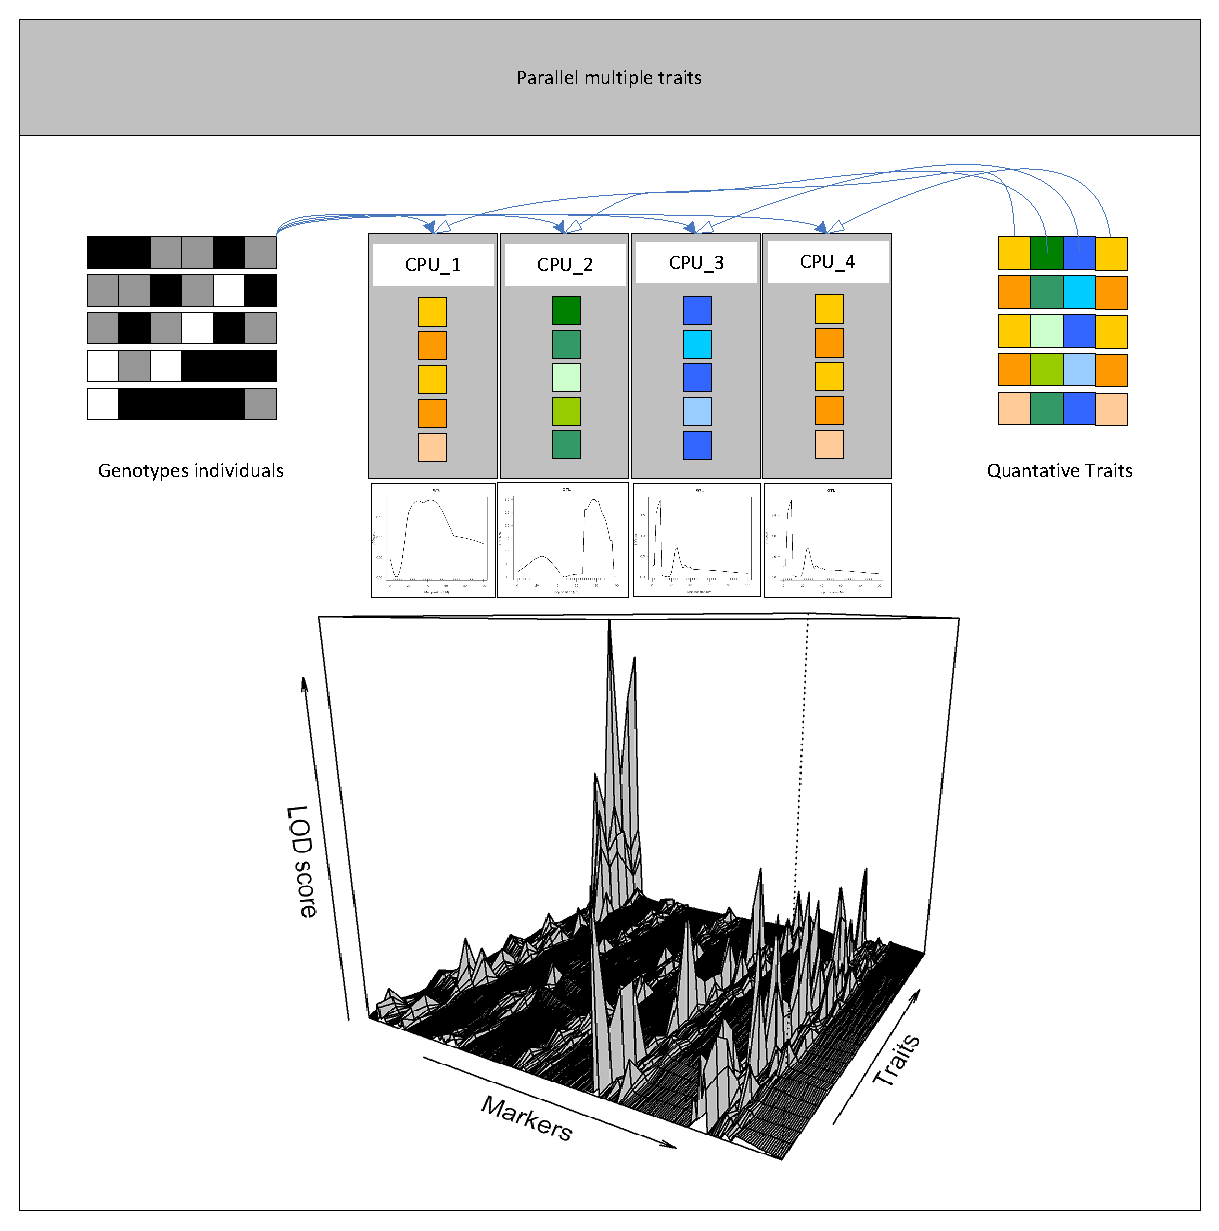
\includegraphics[height=5.0cm,width=10.0cm]{Images/MT_small_newer.eps}}
	  \caption{Overview of the way many endophenotypes are analysed using multiple cores. Tasks are split linearly and distributed across available cores ($Here: \# core = \# traits$, with $traits > cores$ traits are batched into jobs, which are then distributed across cores.)}
	  \label{fig:MTstrait}
	\end{figure}
	
	\begin{figure}[ht]
	  \hfill
	  \fbox{\includegraphics[height=8.0cm,width=12.0cm]{Images/MTperm.eps}}
	  \caption{Overview of the way many endophenotypes permutation using multiple cores. Tasks consist of a single permutation of the data keeping trait correlation intact. Tasks are split linearly and distributed across available cores ($Here: \# core = \# traits$, with $traits > cores$ traits are batched into jobs, which are then distributed across cores.)}
	  \label{fig:MTperm}
	\end{figure}
	
	\begin{figure}[ht]
	  \hfill
	  \fbox{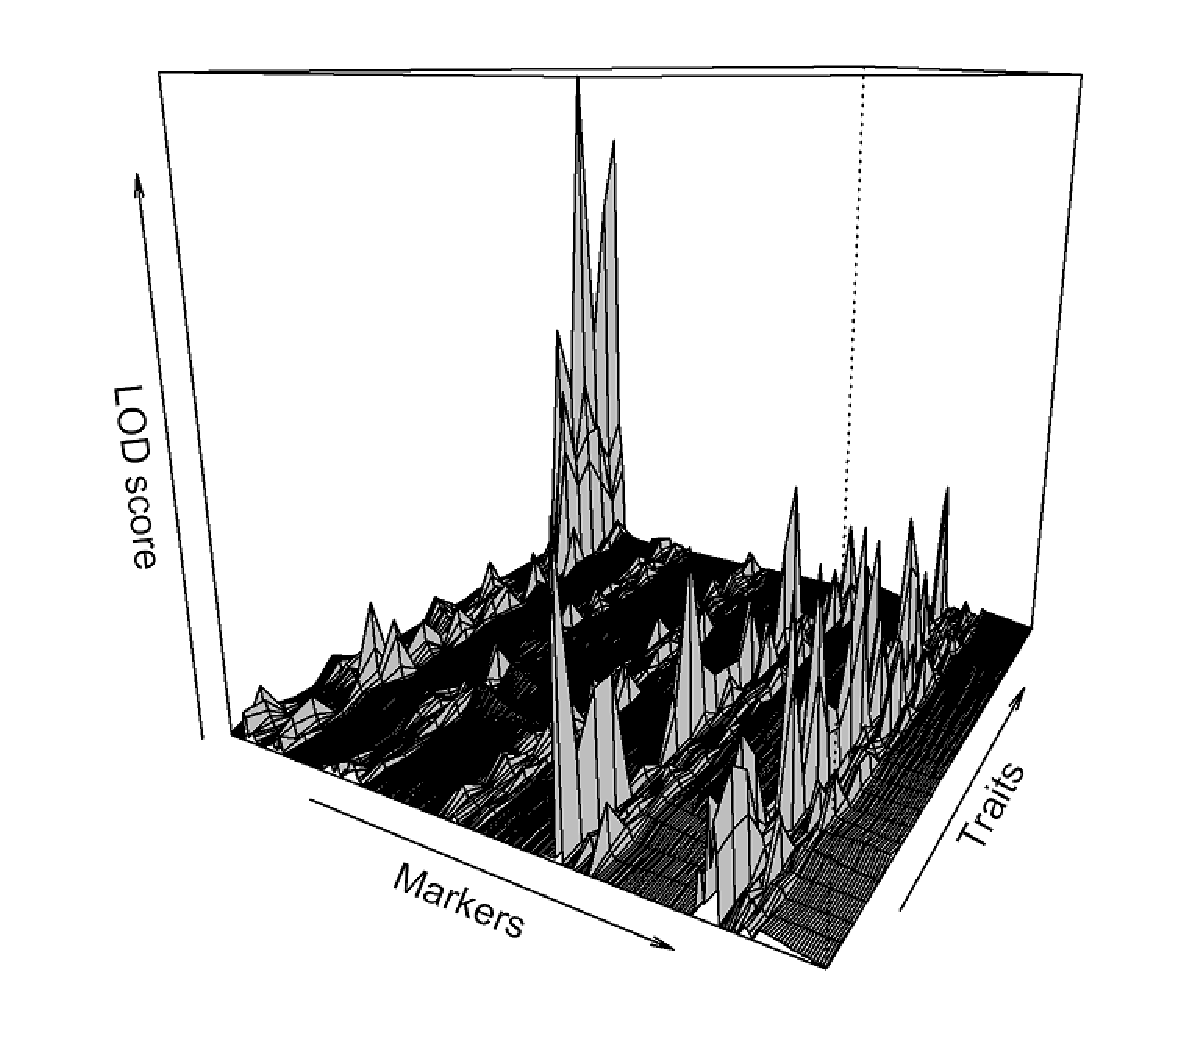
\includegraphics[height=8.0cm,width=12.0cm]{Images/multi3d.eps}}
	  \caption{Example of new ploting routine: Many endophenotypes analyses on 24 traits of the example dataset: "multitrait", displayed in 3D mode}
	  \label{fig:FigureThreeD}
	\end{figure}
	
	\begin{figure}[ht]  
	  \hfill
	  \fbox{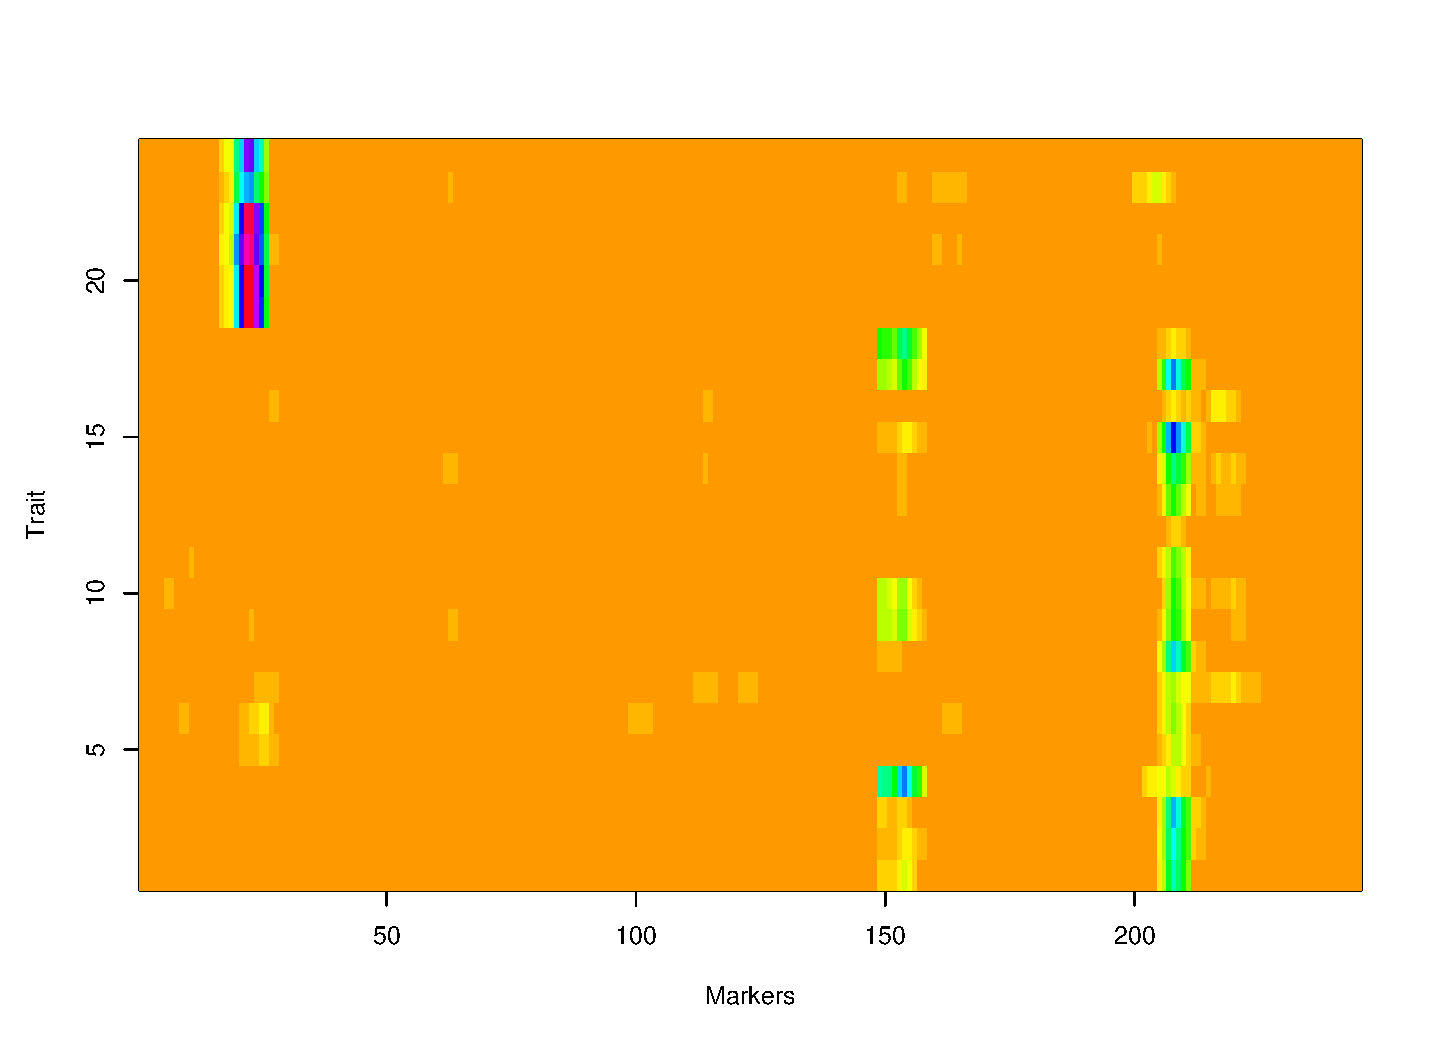
\includegraphics[height=8.0cm,width=12.0cm]{Images/multiHeat.eps}}
	  \caption{Example of new ploting routine: Many endophenotypes analyses analysis on the 24 traits of the example dataset: "multitrait", as a heatmap}
	  \label{fig:FigureHeat}    
	\end{figure}
	
	\begin{figure}[ht]  
	  \hfill
	  \fbox{\includegraphics[height=8.0cm,width=12.0cm]{Images/bootstrap12500.eps}}
	  \caption{Example of new ploting routine: Bootstrap analysis on trait 6 of the example dataset: "multitrait". In this picture the dashed green line represents a 5\% significance threshold, the blue a 10\%.}
	  \label{fig:FigureBoot}
	\end{figure}
	
	\begin{figure}[ht]
	  \hfill
	  \fbox{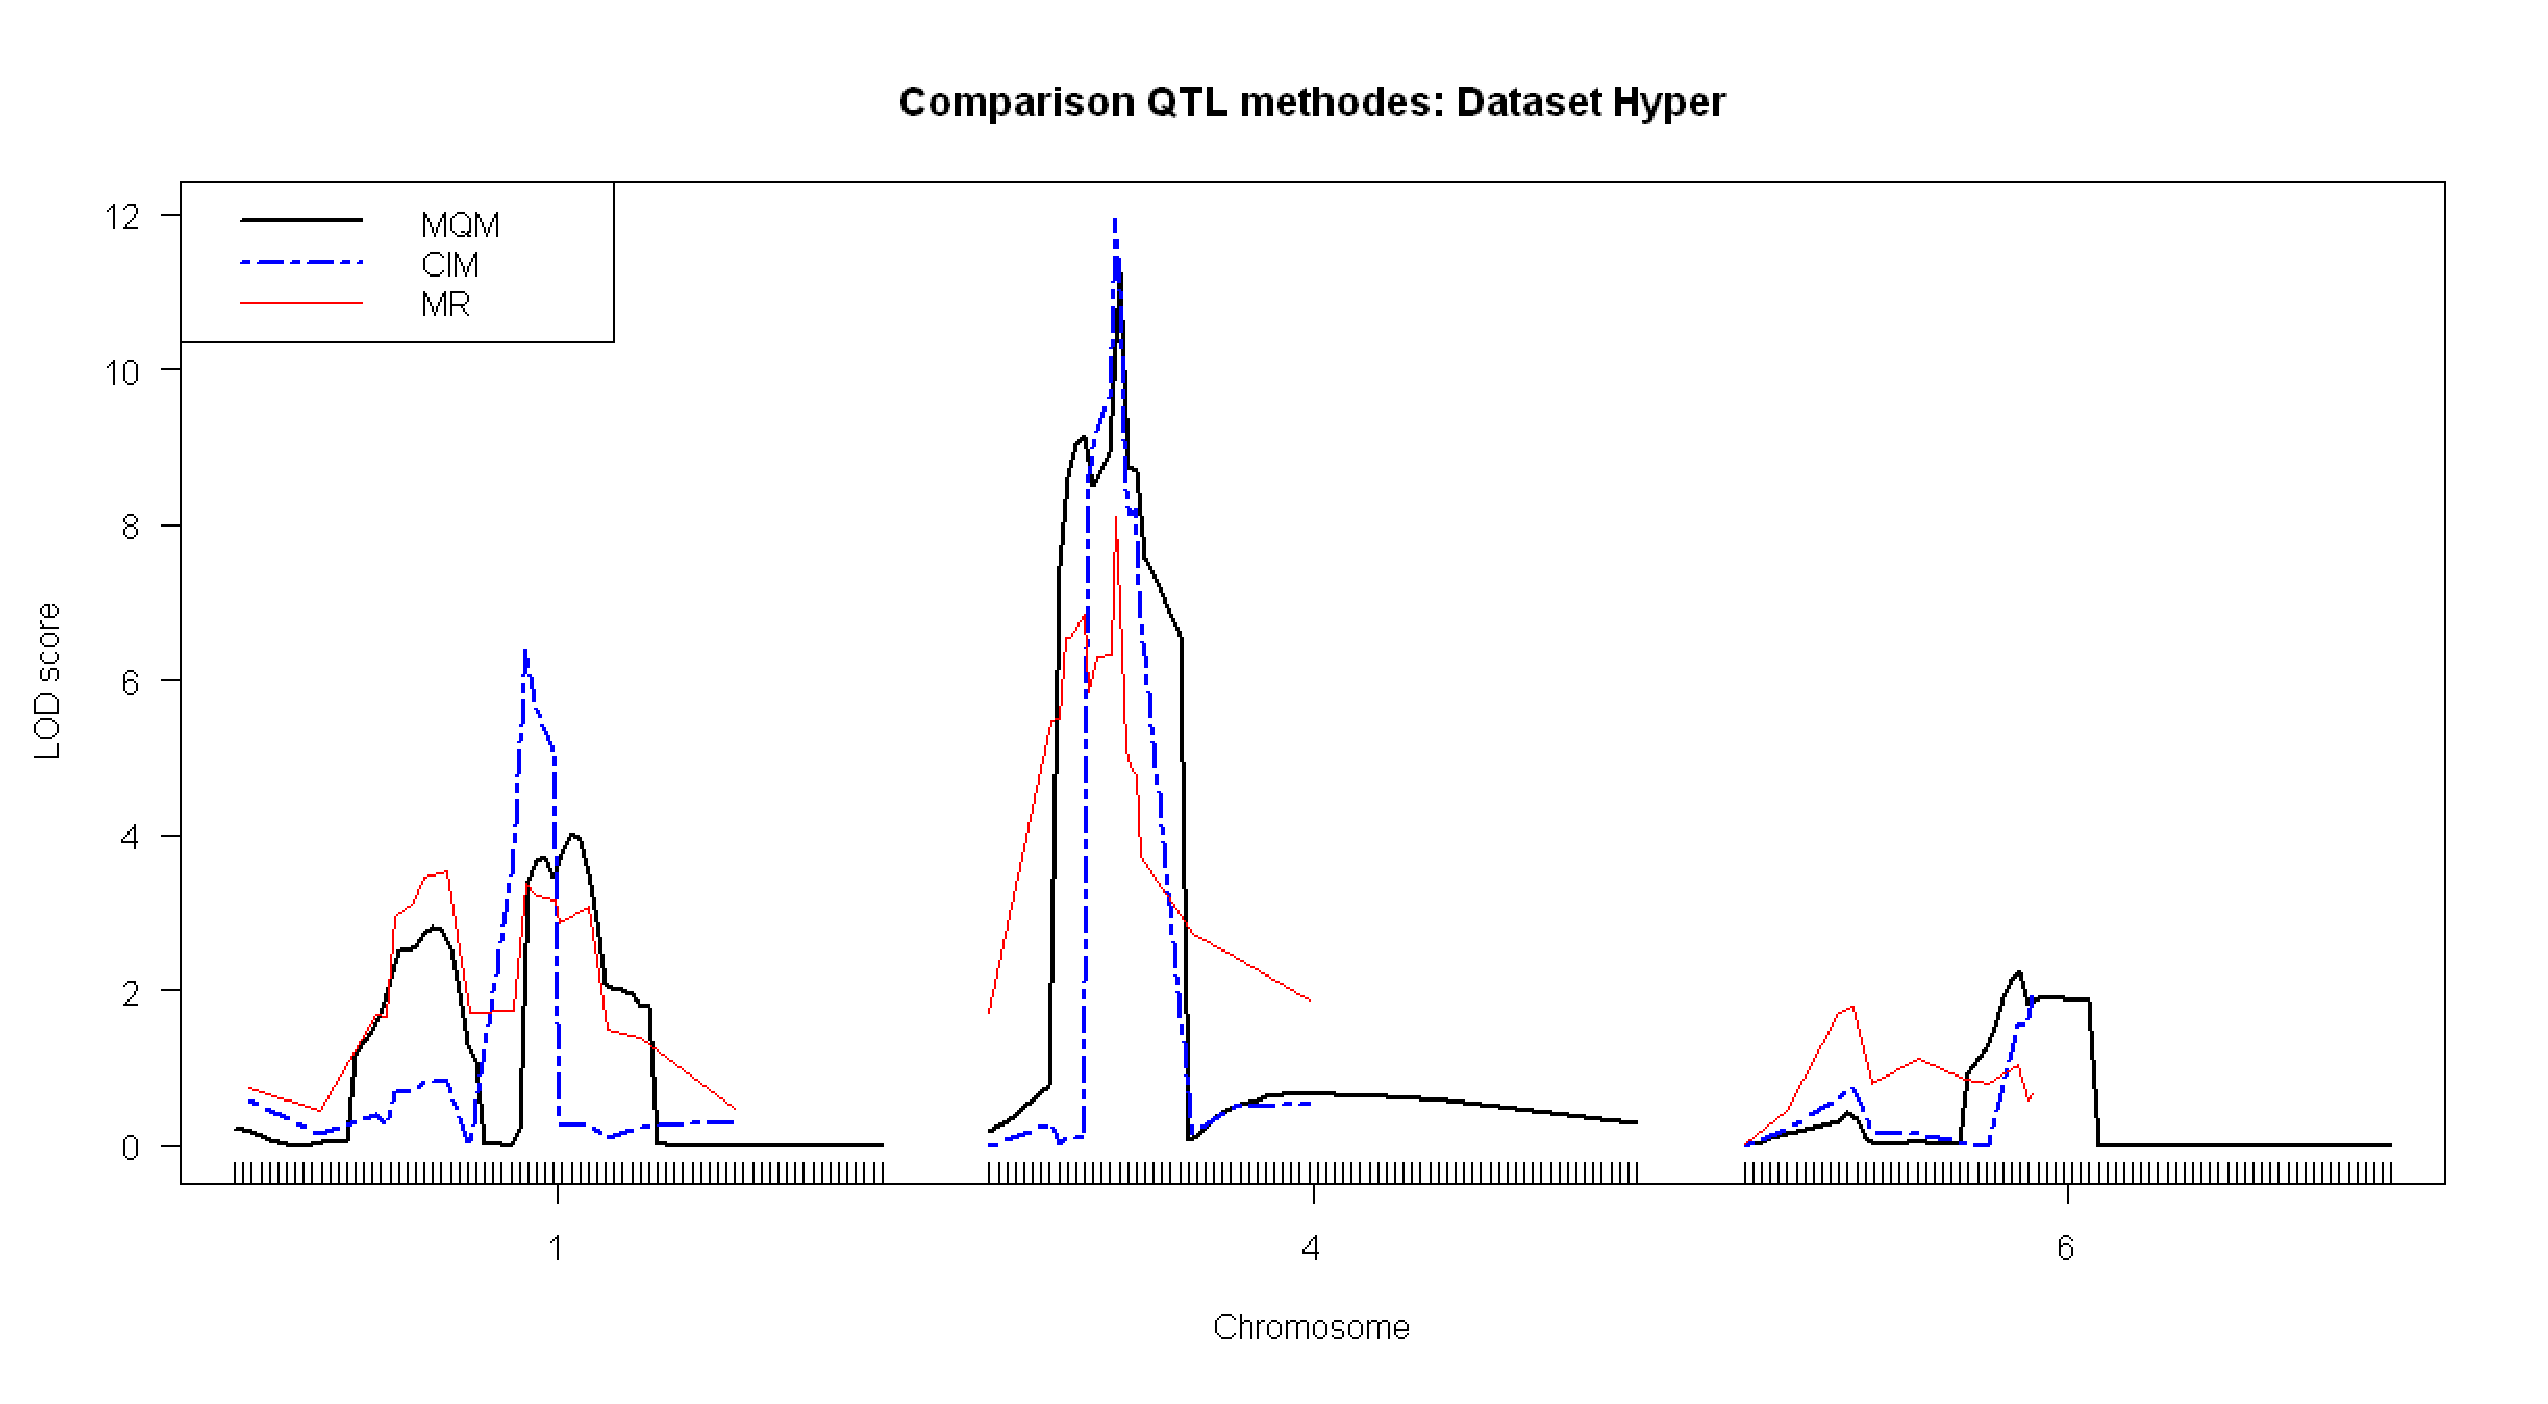
\includegraphics[height=8.0cm,width=12.0cm]{Images/DatasetHyper.eps}}
	  \caption{MQM in comparison with other QTLmapping methods (CIM, MR) using the dataset: "hyper". Using MQM we set cofactors every third marker, and do backward selection using a windowsize of 15 Cm. CIM also uses a window of 15Cm}
	  \label{fig:FigureHyper}
	\end{figure}
	
	\begin{figure}[ht]
	  \hfill
	  \fbox{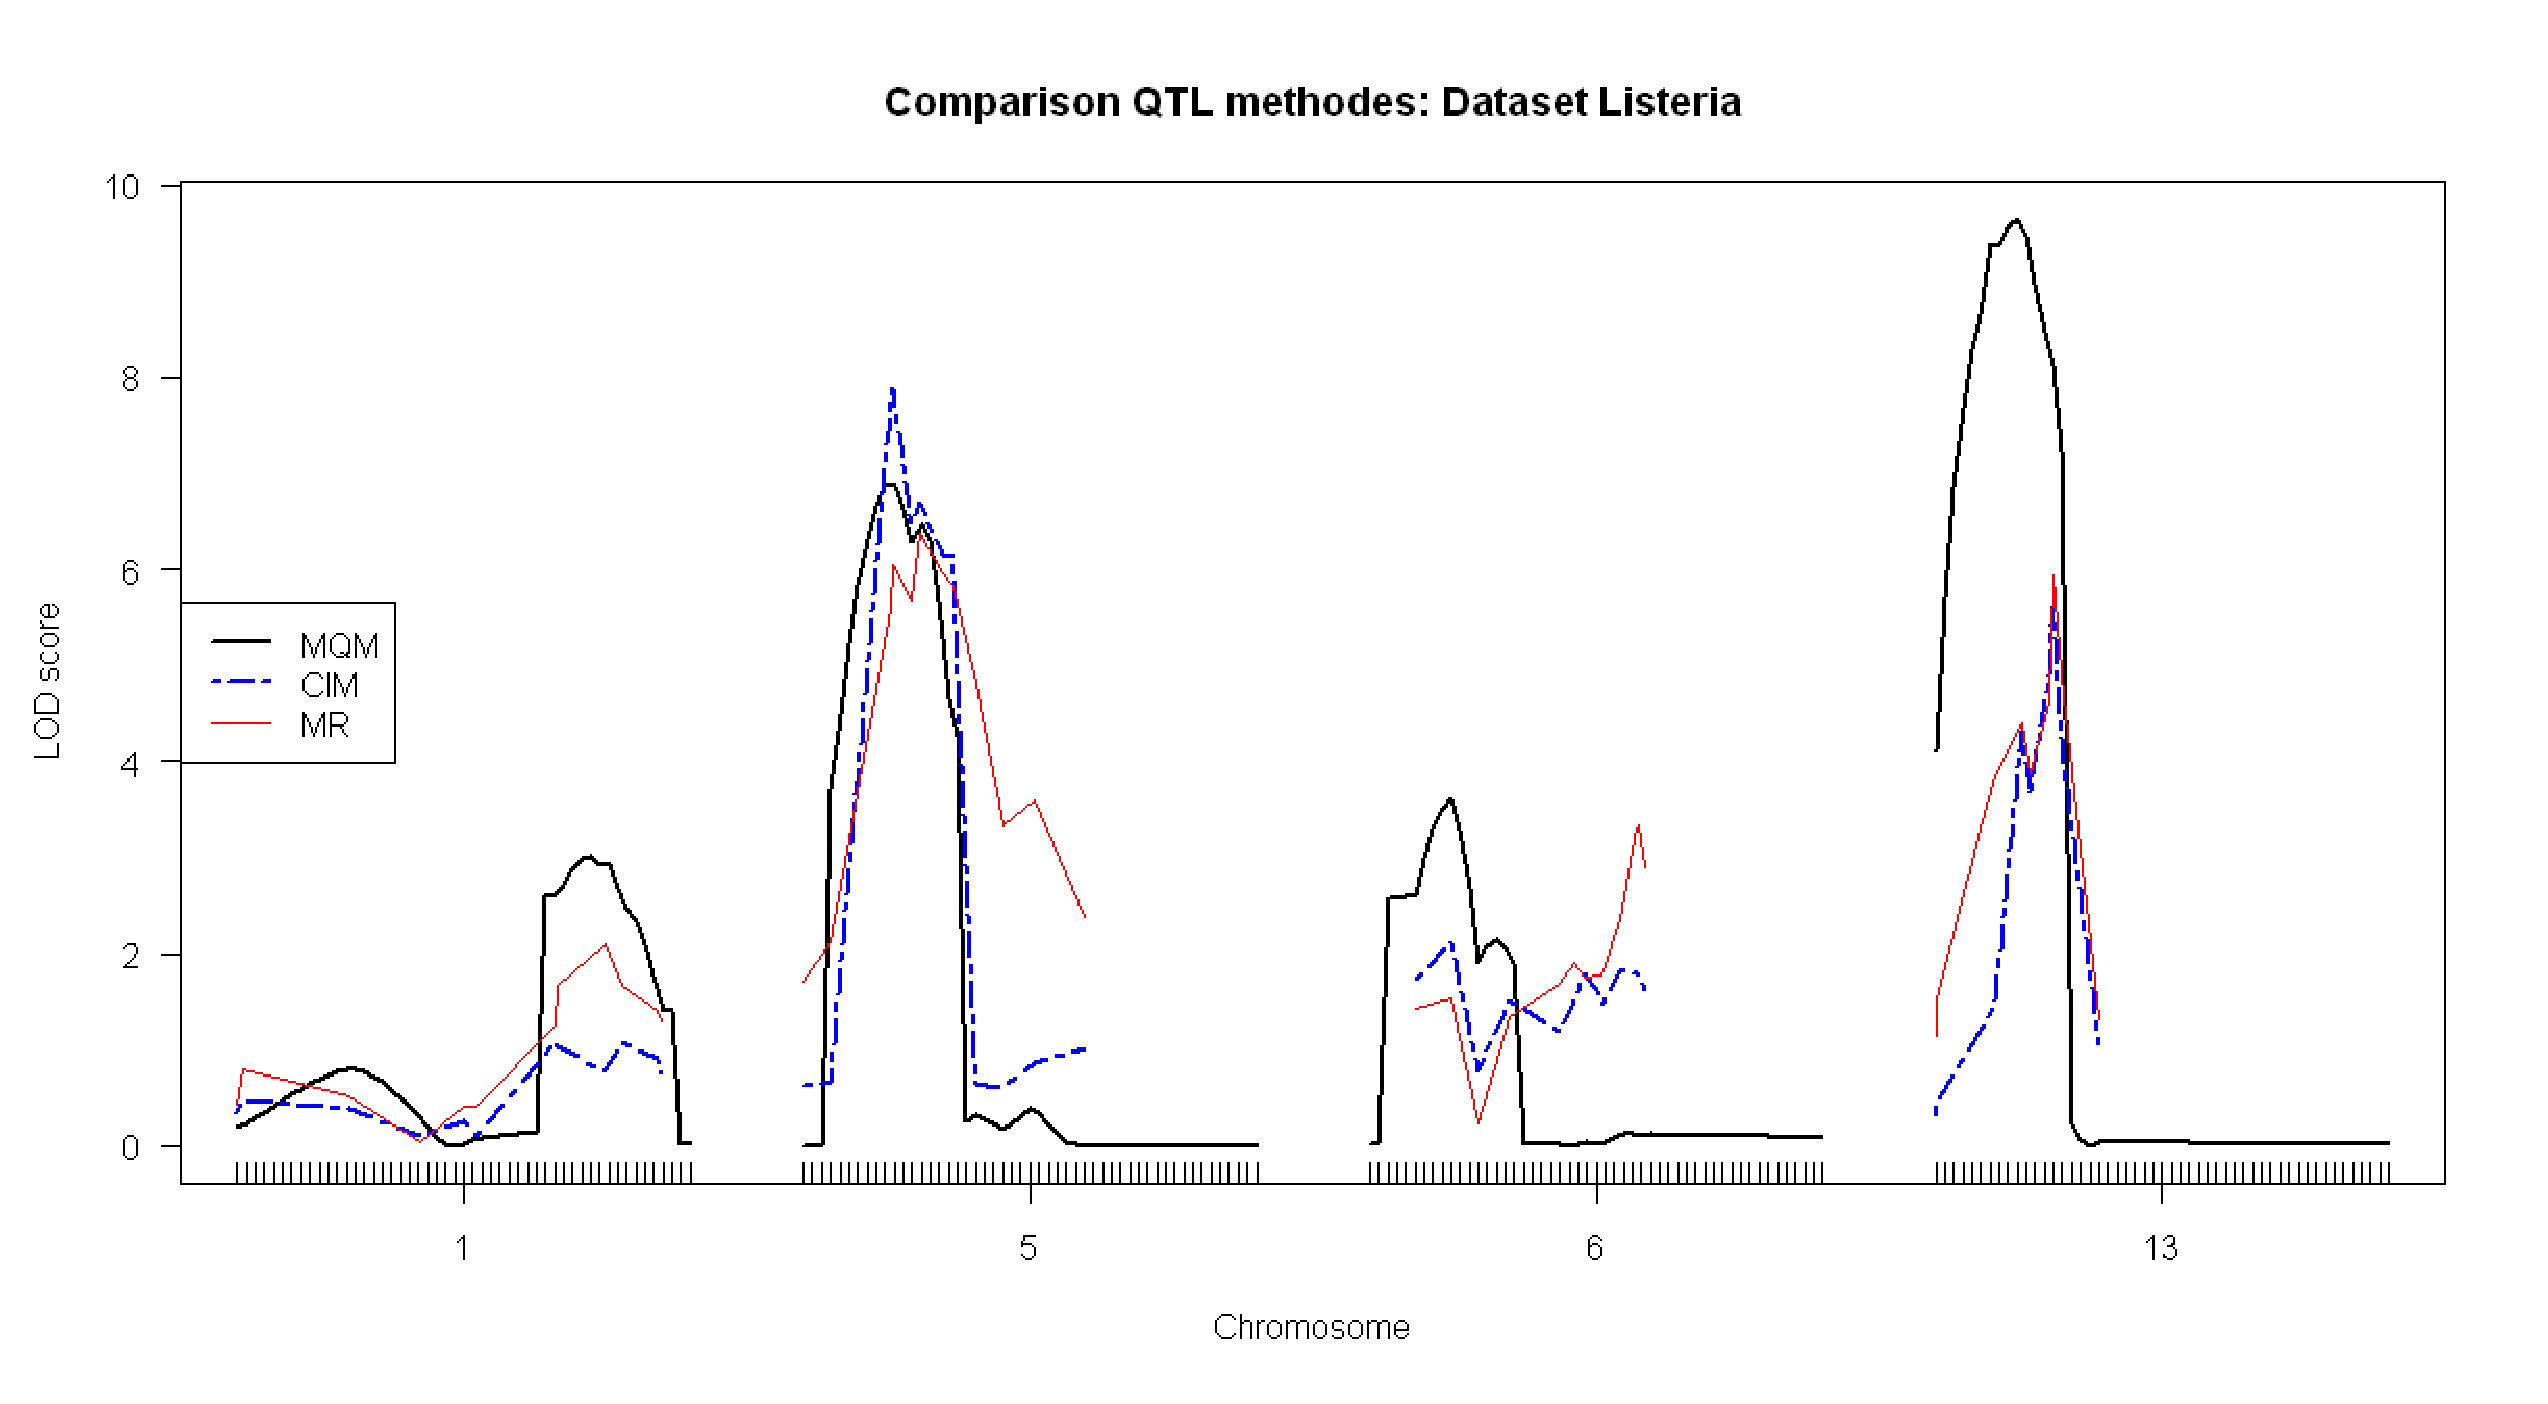
\includegraphics[height=8.0cm,width=12.0cm]{Images/DatasetListeria.eps}}
	  \label{fig:FigureListeria}
	  \caption{MQM in comparison with other QTLmapping methods (CIM, MR) using the dataset: \"listeria\". Using MQM we set cofactors every even marker, and do backward selection using a windowsize of 15 Cm. CIM also uses a window of 15Cm}
	\end{figure}
	
	\begin{figure}[ht]
	  \hfill
	  \fbox{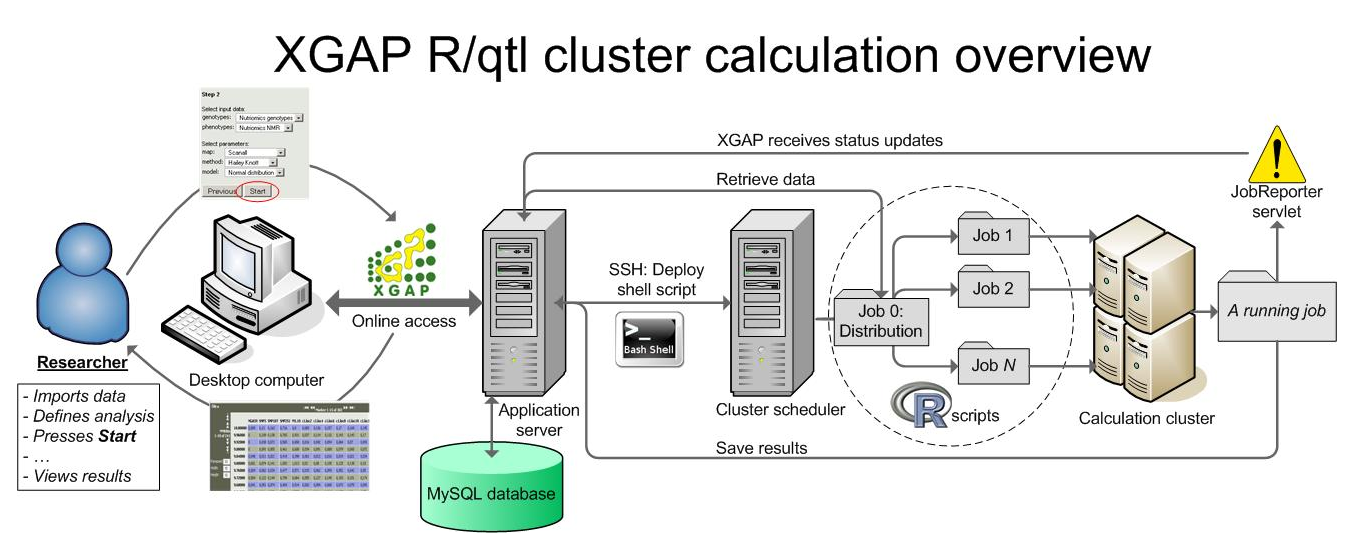
\includegraphics[height=6.0cm,width=12.0cm]{Images/Cluster_Layout.eps}}
	  \label{fig:FigureCluster}
	  \caption{Clusterlayout used at GBIC to do HPC analysis of QTLs using an opteroncluster controlled from the webinterface of a molgenis databaseserver}
	\end{figure}
	
	\begin{figure}[ht]
	  \hfill
	  \fbox{\includegraphics[height=6.0cm,width=12.0cm]{Images/taskviewer.eps}}
	  \label{fig:FigureTaskman}
	  \caption{Overview of the tasmanager plugin. Seen here are different tasks that have been submitted to the cluster. For an overview of the statuscolors see table \ref{tbl:tabelSTATUS}}
	\end{figure}
\end{document}
